% !TEX root =../main.tex

\chapter{Theoretischer Hintergrund und Konzepte}


\section{Social Network}

In den folgenden Abschnitten wird untersucht, wie der Begriff Social Network definiert ist und welche Konzepte von sozialer Netzwerke im Rahmen dieser Arbeit verwendet werden können.


\subsection{Definition Social Network}

% TODO: Zitate überprüfen. Groß- und Kleinschreibung sowie Satzzeichen scheinen nicht korrekt zu sein.

Nach \textcite[S. 2]{aggarwal:sn} \glqq in general, a social network is defined as a network of interactions or relationships, where the nodes consist of actors, and the edges consist of the relationships or interactions between these actors.\grqq \textcite{aggarwal:sn} meint \glqq the concept of social network is not restricted to the specific case of an internet- based social network such as Facebook, such interactions may be in any conventional or non-conventional form, whether they be face to face interactions, telecommunication interactions, email interactions or postal mail interactions\grqq


\subsection{Anwendbare Konzepte Sozialer Netzwerke}

Soziale Netzwerke existierten, um die Bedürfnisse bestimmter Personen zu erfüllen. Sie können anhand ihrer Funktionen wie folgt klassifiziert werden.

\begin{description}
\item[Auf Basis menschlicher Interaktion:] Dazu zählen allgemeine soziale Netzwerke wie Facebook und Myspace, berufliche Netzwerke wie LinkedIn oder Partnervermittlungen wie Parship.
\item[Auf Basis von Blog-Publishing und User-Attention Services:] Als Beispiele sind hierfür Twitter und Follow 5 zu nennen.
\item[Auf Basis von Content Sharing:] Netzwerke welche primär dem Teilen von Inhalten dienen sind beispielsweise Flickr, YouTube oder Delicious.
\item[Auf Basis von Echtzeit-Kommunikation:] Beispiele für soziale Netzwerke mit einem Fokus auf Echtzeit-Kommunikation sind WhatsApp und Skype.

Bei der Echtzeit-Kommunikation gibt es viele Möglichkeiten Informationen zu versenden. Beispiele hierfür sind Text (Instant Messenging), Sprache oder Video. Die Vorteile sind, dass das Senden und Erhalten von Information nahezu ohne Verzögerung geschieht.

Die Akteure welche Facebook nutzen, können unterschiedliche Ausprägungen besitzen. Bei einem Facebook-Account kann es sich z. B. um einen persönlichen Account in Form einer persönlichen Seite handeln. Facebook kann aber darüber hinaus auch als Business-Homepage, kommerzielles Werbekonto oder Business-Management-Plattform genutzt werden, um Events, Aktivitäten und Veranstaltung zu organisieren, beziehungsweise Nachrichten zu kommunizieren.

% TODO: Quelle Chara C der Datei litertur.bib hinzufügen und hier referenzieren.
% TODO: Groß- und Kleinschreibung innerhalb des Zitats kontrollieren.
Expert Discovery in Networks ( Chara C, Social network data analytics, Seite 11) \glqq{}Social networks can be used as a tool in order to identify experts for a particular task. Given the activities of candidates within a context, we first describe methods for calculating the level of expertise for each of them. Many complex tasks often require the collective expertise of more than one expert.\grqq

% TODO: Quelle für Zitat hinzufügen.
\glqq{}Social Tagging:  much of the interaction between users and social networks occurs in the form of tagging, in which users attach short descriptions to different objects in the social network, such as images, text, video or other multimedia data.\grqq

Randoms walks and their Application in Social Networks. Ranking is one of the most well Kown methods in web search. Ranking Users in Social Networks with Higher-Order Structures:

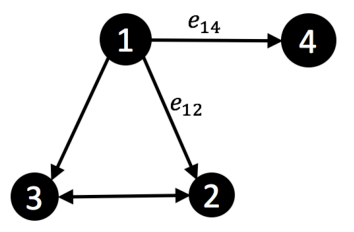
\includegraphics[width=0.3\textwidth]{bilder/social-network-users.png}

Nutzer 1 folgt bei dem dargestellten Sozialen Netzwerk  gleichzeitig den Nutzern 2, 3 und 4. Allerdings existieren hier Unterschiede. Nutzer 1 wird Nutzer 2 mehr als Nutzer 4 vertrauen. Der Grund dafür liegt darin, dass ein Nutzer dem Nutzer 1 folgt, ebenfalls dem Nutzer 2 folgt. Auf der Gegenseite kann Nutzer 4 keine weiteren Nutzer vorweisen, die ihm folgen.

% TODO: Gewünschte Aussage der folgenden Abschnitte muss herausgearbeitet werden. Im Moment leider schwer zu verstehen.
Eine wichtige Funktion innerhalb von sozialen Netzwerken ist das vergeben von Empfehlungen. So ist beispielsweise in Netflix ein System für das Empfehlen von Filmen integriert. Dieses System nutzt die durch Nutzer angesehenen Filme und deren Bewertungen.
% TODO: Quelle in literatur.bib eintragen und hier referenzieren.

Node (User) classification in social Networks. Particular product, and it may be desirable to use the attribute and structural information in the network in order to learn other nodes which may also be interested in the same product. Social networks also contain rich information about the content and structure of the network, which may be leveraged of this purpose.( Laut Charu C Seite 10 An Introduction) Z. B. zwei Nutzer sind miteinander in einem sozialen Netzwerk verbunden. Es ist wahrscheinlich, dass die Knotenbeschriftungen ebenfalls korrelierend sind.

Interaktionen führen dazu, dass verschiedene Akteure sich in ihrem Verhalten gegenseitig beeinflussen. Ein klassisches Beispiel dafür wäre eine virale Marketing Kampagne, bei der wir die Nachrichten zwischen miteinander verbundenen Teilnehmern in einem sozialen Netzwerk nutzen, um die Informationen über die verschiedenen Teile des Netzwerks zu verbreiten.
\end{description}


\section{Social Media}

In den folgenden Abschnitten werden die Definition von Social Media dargelegt und die Konzepte von Social Media untersucht, die im Rahmen dieser Arbeit angewendet werden können.


\subsection{Definition Social Media}

Laut \textcite[S. 8]{turban:sc} kann Social Media als Inhalt definiert werden, welcher durch Nutzer, mit Hilfe von Web 2.0 Plattformen, erzeugt wird. Das Erstellen dieser Inhalte dient hierbei laut \textcite[S. 8]{turban:sc} hauptsächlich dazu Meinungen, Erfahrungen und Erkenntnisse auszutauschen.


\subsection{Anwendbare Konzepte von Social Media}

\begin{itemize}
\item Die Philosophie von miteinander verbundenen Personen \parencite[S. 8]{turban:sc}
\item Nutzer generieren, kontrollieren, nutzen und verwalten Inhalte zu geringen
oder keinen kosten \parencite[S. 8]{turban:sc}
\item Nutzer stellen den eigentlich bereitgestellten Wert bereit, während Betreiber lediglich eine Plattform anbieten, um dies zu ermöglichen  \parencite[S. 8]{turban:sc}
\item Geringe Barrieren für Nutzer, um sich an der Bereitstellung von Inhalten zu beteiligen \parencite[S. 8]{turban:sc}
\end{itemize}


\section{e-Commerce}

Nachfolgend werden der Begriff e-Commerce definiert, sowie Konzepte des e-Commerce untersucht, die für die Arbeit anwendbar sein könnten.


\subsection{Definition  e-Commerce}

Nach \textcite[S. 20]{merz:e-commerce} ist e-Commerce  \glqq die Unterstützung von Handelsaktivitäten über Kommunikationsnetze\grqq. E-Commerce ist der Einsatz von Kommunikationsprotokollen, Sicherheitsinfrastrukturen, digitalem Geld, Electrpmoc Shopping -malls und Datenaustausch….\grqq


\subsection{Anwendbare Konzepte des e-Commerce}

\begin{description}
\item[Online Auktionen:] Aus \textcite[Kapitel 4: Wirtschaftliche Bedeutung von Ebay, S. 71]{hinneburg} \glqq da nicht die online -Auktionsmärkte selbst, sondern nur ihre Mitglieder Waren zum Verkauf anbieten, entscheidet die jeweilige Mitgliederzahl über die Quantität und Vielfalt des Warenangebotes eines Auktionsmarktes. Andererseits lohnt sich der Verkauf von Waren nur, wenn zahlreiche Käufer den Auktionsmarkt frequentieren.\grqq ~\textcite[S. 72]{hinneburg} hat noch konkret beschrieben, wie eine Auktion abläuft.

In Abbildung \vref{fig:laufende-auktionen} ist die Anzahl der laufenden Auktionen auf den zehn bedeutendsten deutschsprachigen Auktionsmärkten im Internet dargestellt.

\item[Gebrauchte Produkte verkaufen: ] Über Ebay Kleinanzeigen verkaufen viele Menschen Dinge, die sie nicht mehr benötigen – mit häufig äußerst kuriosen Anzeigen und witzigen Dialogen. Ein Verkäufer lädt ein Bild des Produkts mit entsprechenden Informationen wie Maßen und Preis hoch. Findet ein potentieller Käufer diese Anzeige interessant, tauschen sich Käufer und Verkäufer über weitere Details aus. In den meisten Fällen holt der Käufer das Objekt der Begierde beim Verkäufer ab. Beide Seiten profitieren, denn der Verkäufer hat wieder Platz in der Wohnung und bekommt Geld. Der Käufer hat für einen günstigeren Preis sein Wunschobjekt bekommen.

\item[Bewertungen von Produkten: ] Bei dem Online-Versandhändler Amazon kann man nach dem Kaufen eines Produktes eine Bewertung abgeben und Kommentare verfassen. Die Bewertung nutzt eine Skala von 1 - 5 Sternen und spiegelt die Zufriedenheit des Kunden wieder. Die Kommentare beschreiben konkret wie ein Käufer sein Kauferlebnis und das erworbene Produkt empfindet. Die Bewertung und Kommentare sind ein Teil der Dienstleistung, da sie anderen Nutzern helfen Produkte auszuwählen.
\end{description}

\begin{figure}
	\centering
	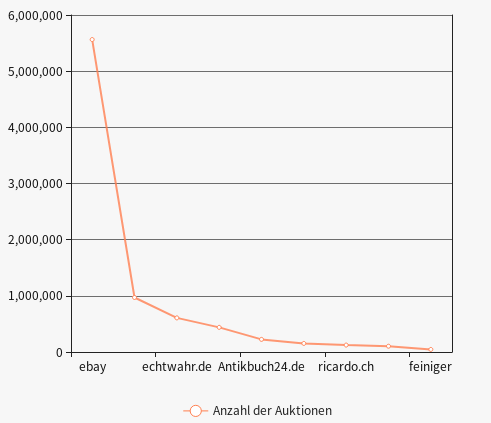
\includegraphics[width=0.7\textwidth]{bilder/laufende-auktionen.png}
	\caption[Laufende Auktionen]{Laufende Auktionen (Quelle: www.auktionssuche.de)}
	\label{fig:laufende-auktionen}
\end{figure}


\section{Social Commerce}

In den nachstehenden Abschnitt wird zuerst der Begriff Social Commerce definiert. Anschließend wird untersucht, welche Konzepte des Social Commerce in dieser Arbeit angewendet werden können.


\subsection{Definition Social Commerce}

Social Commerce basiert auf den Konzepten von e-Commerce und Social Media. \textcite[S. 8]{turban:sc} beschreiben: \glqq{}The figur shows that social Commerce is created from the integration of e-commerce and e-marketing using  Web 2.0/social media applications.\grqq{} Es nutzt soziale Netzwerke, wie z.B. Twitter, Blogs oder YouTube, um Produkte durch soziale Interaktionen und vom Benutzer bereitgestellte Inhalte zu bewerben. Es ist ein effektiver Werbekanal für e-Commerce.


\subsection{Anwendbare Konzepte des Social Commerce}

Die Einkaufsnachfrage des Nutzers entsteht unter dem Einfluss von anderen Nutzern. Es besteht eine starke Korrelation zwischen den Bedürfnissen eines Nutzers und den Bedürfnissen anderer Nutzer. Word-of-mouth (WOM) advertising (Marketing communication) is \glqq{}an unpaid form of promotion in which satisfied customers tell other people how much they like a business, product, or Service\grqq{}, \glqq{}Reaserch has revealed that customers are inclined to believe WOM rather than company generated promotions\grqq{} \parencite[S. 58]{turban:sc} Interessen und Wünsche werden mit denen von anderen Nutzern geteilt und durch Bewertungen, Kommentare oder Bilder angeregt.

Sozial Commerce leitet Nutzer zu Webshops. Der Einkaufsführer ist der Nutzer selbst. Es basiert auf der Erfahrung des Benutzers, Produktinformationen zu teilen, Produkte zu überprüfen, Produkte anzuzeigen und Produkte zu teilen, um mit anderen Nutzern zu interagieren und soziale Beziehungen mit sozialen Attributen herzustellen.

Die Plattform erstellt die Community. Sie bietet für viele Nutzer von Online-Shopping einen Ort, um miteinander Einkaufsinformationen und Erfahrungen auszutauschen und gleichgesinnte kennenzulernen. Dadurch kann die Beziehung zwischen den Nutzern verstärkt werden. Die User Stickiness des Benutzers und die Stickiness zwischen der Webseite und den Nutzern wird erhöht.

\begin{itemize}
\item Eine community-basierte Social Commerce -Plattform wie Facebook oder Twitter implementiert Präzisionsmarketing
\end{itemize}

Gewinnmodell: a) Werbung, 80\% Anteil; b) Kommission; c)  Mehrwertdienste, Sammeln von Beiträgen vom VIP, um kostenpflichtige Dienste und spezielle Dienste zu erhalten; d)  Virtueller Warenverbrauch Plug-in-Anwendungsfreigabe von Drittanbietern

Erweiterte Gewinnmodelle:

\begin{description}
\item[Werbung] Social Commerce kann Unternehmen helfen, Data Mining und Analyse von Benutzerpräferenzen und potenziellen Bedürfnissen durchzuführen und Online-Werbung für eine bestimmte Zielgruppe zu starten.
\item[Fragebögen] Social Commerce kann kostenpflichtige Fragebogenumfragen anbieten. Die Anzahl der Benutzer, die erhoben werden, um Unternehmen bei der Durchführung von professionellen Ermittlungen und Analysen zu unterstützen, hat großen Einfluss auf die Qualität des Ergebnisses.
\item[Zusätzliche Dienste] Einführung des PPC- und Keyword-Bidding-Service und Einführung des SOLOMO-Modells. Solomo ist ein Akronym für Social Local Mobile. Kurz gesagt, das SOLOMO-Modell soll lokalisierte Dienste für Benutzer mit gemeinsamen Bedürfnissen über das Internet bereitstellen und effektiv online und offline integrieren.
\end{description}

Ein wichtiger Faktor im Social Commerce sind Produktbilder: Website-Betreiber stellen kostenlose, herunterladbare Software bereit, die es den Kunden erleichtert, Fotos hochzuladen und Einkaufserlebnisse auszutauschen. Eine solche Software ermöglicht es den Verbrauchern nicht nur, ihre Lieblingsprodukte aufzulisten, sondern auch die Fotos von Einkaufslisten anzupassen und eine Einnahmequelle zu schaffen. Zum Beispiel können diese Webseiten durch den Verkauf von Click-to-Pay-Anzeigen Geld verdienen. Sie können auch eigene marktrelevante Informationen anbieten.


\section{Anwendbare Konzepte des Online Gamings}

Die Spielteilnehmer kooperieren, um eine Aufgabe zu erfüllen. Sie können ein Team bilden oder auch alleine eine Aufgabe erfüllen.

Die Spielszene ist ansprechend und detailliert.

% TODO: Bitte aussage dieses Stichpunkts deutlicher machen. Im Moment nur schwer zu verstehen.
Virtuelle Güter können verkauft werden. Diese schalten neue Fähigkeiten und Funktionen frei und sind bei Free-to-Play spielen die eigentliche Einnahmequelle der Entwicklerfirmen.

Es gibt Communities für Gamer, um Nachrichten zu veröffentlichen und Erfahrungen auszutauschen \parencite[S. 126]{warmelink}.


\section{Vergleich beliebter Webshops}

Tabelle \vref{tab:variable-breite} nutzt eine Untermenge der herausgearbeiteten Konzepte, um eine Auswahl an populären Webshops gegenüberzustellen.

\begin{table}[htbp]
\centering
\begin{tabular}{l l l l l l}
\toprule
Kriterien				& Amazon	& Ebay	& Alibaba	& Bandcamp	& Zalando\\
\midrule
Nutzer-Community		& nein		& nein	& ja		& ja		& nein\\
Online-Kommunikation	& nein		& ja	& ja		& nein		& nein\\
Vielfältige Produkte	& ja		& ja	& ja		& ja		& nein\\
Pay by others			& nein		& nein	& ja		& nein		& nein\\
Bewertungen				& ja		& nein	& ja		& ja		& ja\\
\bottomrule
\end{tabular}
\caption{Tabelle mit variabler Spaltenbreite}
\label{tab:variable-breite}
\end{table}
